\section{Arsitektur Sistem}
\label{sec:arsitektur}

\subsection{Gambaran Umum}

Sistem dibangun sebagai sekumpulan service yang dikemas dan dijalankan
terpisah melalui Docker Compose. BMKG dan PVMBG berperan sebagai \textit{mock
service}. Aggregator melakukan polling ke kedua sumber, memetakan respons ke
format kanonik \textit{HazardEvent}, menyimpannya pada Canonical Store, dan
menerbitkan event baru ke message broker.

Client downstream tidak membaca database secara langsung. Permintaan data masuk
melalui Client-Facing API, yang memverifikasi token client, menerapkan filter
hak akses, lalu mengambil data dari API internal milik Aggregator. Event baru
diterima consumer independen untuk kebutuhan dashboard dan notifikasi.
Diagram arsitektur sistem ditunjukkan pada Gambar~\ref{fig:arsitektur-sistem}.

\begin{figure}[H]
  \centering
  % Render docs/figures/arsitektur-sistem.puml lalu simpan hasilnya sebagai
  % docs/figures/arsitektur-sistem.png.
  \IfFileExists{figures/arsitektur-sistem.png}{%
    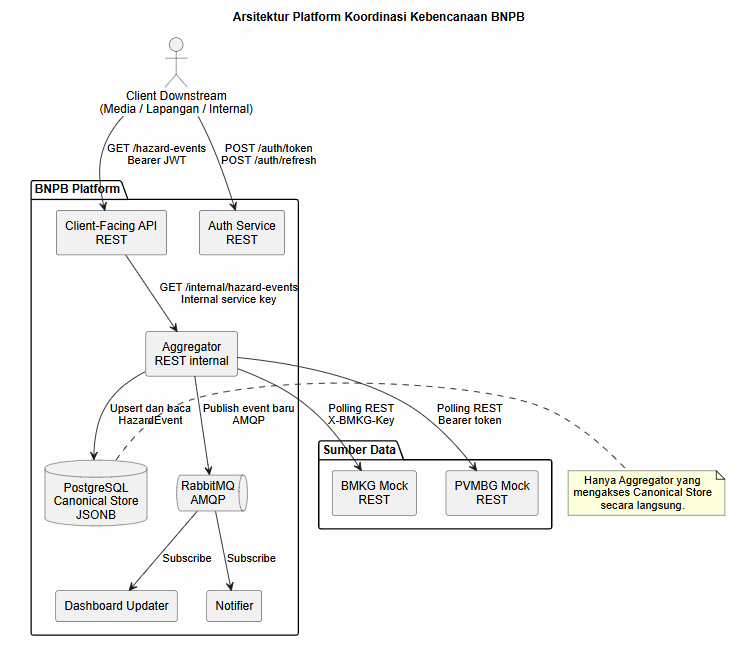
\includegraphics[width=\textwidth]{figures/arsitektur-sistem.png}%
  }{%
    \fbox{\parbox[c][5cm][c]{0.9\textwidth}{\centering
      Placeholder diagram arsitektur sistem}}%
  }
  \caption{Arsitektur platform koordinasi kebencanaan BNPB.}
  \label{fig:arsitektur-sistem}
\end{figure}

\subsection{Komponen dan Batas Service}

\begin{table}[H]
  \centering
  \caption{Komponen utama sistem.}
  \label{tab:komponen}
  \begin{tabularx}{\textwidth}{@{}p{0.23\textwidth}p{0.20\textwidth}X@{}}
    \toprule
    \textbf{Komponen} & \textbf{Antarmuka} & \textbf{Tanggung Jawab} \\
    \midrule
    BMKG Mock & REST & Menyediakan data \textit{SeismicEvent} dan
    \textit{TsunamiWarning}; akses menggunakan \texttt{X-BMKG-Key}. \\
    PVMBG Mock & REST & Menyediakan \textit{VolcanicReport},
    perubahan skema, dan simulasi outage; akses menggunakan \textit{Bearer token}. \\
    Aggregator & REST internal & Polling, mapping, penyimpanan
    Canonical Store, serta publikasi event baru. \\
    PostgreSQL & Koneksi database internal & Menyimpan \textit{HazardEvent}
    dengan atribut dinamis pada kolom \texttt{JSONB}; hanya Aggregator yang
    mengaksesnya langsung. \\
    Client-Facing API & REST & Menyajikan data untuk client,
    memvalidasi JWT, dan menerapkan RBAC. \\
    Auth Service & REST & Menerbitkan dan memperbarui token client. \\
    RabbitMQ & AMQP & Broker distribusi event dengan pola fan-out. \\
    Event Consumer & AMQP consumer & Menerima event baru secara
    independen untuk dashboard dan notifikasi. \\
    \bottomrule
  \end{tabularx}
\end{table}

\subsection{Alur Komunikasi dan Data}

Aggregator melakukan polling berkala melalui REST. Kredensial untuk BMKG berupa
API key, sedangkan PVMBG menggunakan \textit{Bearer token}. Respons sumber
dipetakan ke \textit{HazardEvent} dan disimpan oleh Aggregator ke PostgreSQL.
Field dinamis disimpan pada \texttt{attributes} bertipe \texttt{JSONB}.

Setiap event baru yang tersimpan diterbitkan Aggregator ke RabbitMQ. Dashboard
Updater dan Notifier berlangganan melalui broker; Aggregator tidak memanggil
consumer secara langsung. Untuk alur baca, client memperoleh access token dari
Auth Service dan mengirimkannya ke Client-Facing API. Setelah memvalidasi token
dan scope, Client-Facing API memanggil endpoint internal Aggregator dengan
\textit{internal service key}. Dengan demikian, PostgreSQL bukan dependency
langsung bagi Client-Facing API maupun consumer.

\subsection{Teknologi dan Konfigurasi}

Service aplikasi dibangun menggunakan Node.js, TypeScript, dan Fastify.
Komunikasi sinkron menggunakan REST, sedangkan distribusi event memakai RabbitMQ
melalui AMQP. Canonical Store menggunakan PostgreSQL dengan \texttt{JSONB}
untuk menyimpan atribut sumber yang dinamis tanpa penambahan kolom baru.
Tabel~\ref{tab:teknologi} merinci seluruh teknologi yang dipakai beserta
alasan pemilihannya.

\begin{table}[H]
  \centering
  \caption{Teknologi yang digunakan dan alasan pemilihan.}
  \label{tab:teknologi}
  \begin{tabularx}{\textwidth}{@{}p{0.2\textwidth}X@{}}
    \toprule
    \textbf{Teknologi} & \textbf{Alasan Pemilihan} \\
    \midrule
    TypeScript (strict mode) & Tipe statis menangkap ketidakcocokan kontrak
    antar-service saat compile, penting karena tiap domain kepercayaan
    (BMKG, PVMBG, client) punya bentuk payload berbeda. \\
    Fastify & Overhead rendah dan validasi skema bawaan, cocok untuk service
    kecil yang perlu start cepat dan banyak dijalankan sebagai container
    terpisah. \\
    \texttt{pg} & Driver PostgreSQL resmi tanpa lapisan ORM, dipilih agar
    kueri SQL ke Canonical Store (termasuk \texttt{UPSERT} dan filter
    \texttt{JSONB}) tetap eksplisit dan mudah diaudit. \\
    PostgreSQL + \texttt{JSONB} & Mendukung evolusi skema aditif (field baru
    dari sumber langsung masuk ke \texttt{attributes}) tanpa migrasi, sesuai
    kebutuhan Problem 4. \\
    RabbitMQ + \texttt{amqplib} & Exchange bertipe \textit{fanout} memenuhi
    kebutuhan Problem 5: Aggregator menerbitkan event sekali, seluruh
    consumer menerimanya secara independen tanpa Aggregator mengetahui
    siapa saja consumer-nya. \\
    \texttt{jsonwebtoken} & Implementasi JWT standar untuk menerbitkan dan
    memvalidasi access/refresh token client serta domain kepercayaan PVMBG,
    tanpa menulis ulang logika signing/verifikasi sendiri. \\
    \texttt{zod} & Validasi skema environment variable saat startup
    (\texttt{config.ts} tiap service), sehingga konfigurasi yang salah
    membuat service gagal start lebih awal alih-alih gagal diam-diam saat
    runtime. \\
    \texttt{pino} & Logger terstruktur (JSON) dengan dukungan
    \texttt{correlation\_id} lewat \texttt{AsyncLocalStorage}, dipilih agar
    log antar-service bisa ditelusuri dalam satu alur permintaan. \\
    \texttt{vitest} & Test runner cepat dan kompatibel langsung dengan
    TypeScript/ESM tanpa konfigurasi transpiler tambahan, dipakai untuk
    131 unit test di seluruh service. \\
    k6 & Load testing terskrip untuk mengukur throughput dan latensi p95
    pada Problem 2, dengan dukungan skenario VU paralel yang meniru beban
    BMKG-only dan beban campuran. \\
    Docker Compose & Orkestrasi lokal yang mengemas setiap service sebagai
    container terpisah dengan jaringan internal sendiri, selaras dengan
    batas service yang dituntut Problem 4. \\
    \bottomrule
  \end{tabularx}
\end{table}

Seluruh service dijalankan melalui \texttt{docker-compose.yml}. Port, URL
service, credential, interval polling, parameter circuit breaker, koneksi
database, koneksi broker, dan kunci internal dikonfigurasi melalui environment
variable.
